\section{Progettazione}
Durante la fase di progettazione è stata effettuata una scelta fondamentale: i linguaggi da utilizzare. Per consentire una migliore integrazione con le tecnologie assistive di ultima generazione, e per sfruttare al meglio le potenzialità del design Responsive
si è scelto di utilizzare HTML5 e CSS3, in simbiosi con JavaScript e PHP5.

Un ulteriore sicurezza sulla scelta delle tecnologie da utilizzare  ci é stata fornita dal confronto con i \textit{competitors}: effettuano la nostra stessa scelta, come nel caso di \href{www.dolomitisuperski.com}{Dolomiti Superski}.

Grazie all'utilizzo di CSS3 abbiamo potuto svilupare una interfaccia con l'utilizzo dei \verb|display:flex| e \verb|display:grid|.


\subsection{Attori}
Un fruitore del nostro sito web ricade sempre in una delle seguenti 3 categorie: Amministratore, Utente standard, Utente registrato.
\subsubsection{Amministratore}
È la categoria di utenti con più potere, può visitare l'area riservata da cui gestire i prezzi degli skipass e lo stato del comprensorio.
È un account interamente dedicato all'amministrazione, non personale, e pertanto ci si aspetta un utilizzo prevalentemente da Desktop o Tablet. Per questo motivo il link alla pagina Dashboard non è presente nella visualizzazione da Cellulare, ma è sempre raggiungibile al link noto per interventi straordinari.
\subsubsection{Utente standard}
Può usufruire di tutte le funzionalità del sito tranne la prenotazione degli skipass e l'amministrazione.
\subsubsection{Utente registrato}
Questa categoria di utenti ha la possibilità di prenotare online gli skipass, oltre a tutte quelle di un Utente standard

\subsection{Struttura del sito}
Il sito web del comprensorio ha una struttura piuttosto semplice, raggiungendo al massimo 3 livelli di profondità.
Tutti i contenuti principali sono accessibili dal menu di navigazione primario: questo rende l'esperienza nel sito estremamente intuitiva e adatta alla fruizione in qualsiasi situazione, anche lungo il bordo di una pista da sci.

\subsubsection{Menù}
Questo elemento costituisce il principale modo di navigare il sito web. Il menu è disponibile in 3 layout diversi a seconda della larghezza dello schermo con il quale viene visualizzato: semplice lista di links disposta orizzontalmente da \textbf{Desktop}, una lista comprimibile disposta verticalmente da \textbf{Tablet} e dei pulsanti con icone da \textbf{Mobile}.
Il menu occupa in ogni caso tutta la larghezza dello schermo per sfruttarne al meglio le potenzialità, ed è pensato in modo da eliminare i link circolari.
\paragraph{Implementazione}\label{MenuPrinc}
Per la realizzazione di un menu in grado di mutare forma, i links sono stati inseriti in un \verb|flexbox| così da poterne facilmente cambiare l'orientamento. Inoltre l'utilizzo di fogli di stile appositi ha consenito la visualizzazione differente e l'aggiunta di icone.

Per quanto riguarda il pulsante che permette di espandere e comprimere il menu nella visualizzazione intermedia, è stato realizzato mediante bottone e appositi tag di accessibilità, come \verb|aria-expanded|. Il comportamento è delegato al file JavaScript.
\subsubsection{Breadcrumb}
La breadcrumb del nostro sito è minimale ma svolge comunque un ruolo essenziale all`interno del sito, consentendo di sapere constantemente dove ci si trova ed i passaggi effettuati per arrivare in quel punto.
\subsubsection{Contenuti}
I contenuti del sito assolvono due compiti: informare potenziali clienti a riguardo del comprensorio, e fornire gli strumenti ai potenziali clienti per diventare dei clienti effettivi.

I contenuti delle pagine sono stati progettati in modo da avere sempre un'alternativa testuale per consentirne la fruizione da parte di tutte le categorie di utenti.

Ai fini della leggibilità e usabilità, la pagina "Mappa" è raggiungibile solamente nella visualizzazione desktop, mentre nei layout mobile `consultabile dalla pagina "Il nostro comprensorio".
Negli schermi più piccoli non risultava pratico premere i link presenti sulla mappa, che pertanto diventa un immagine statica.
\paragraph{Home} Nella pagina Home si trovano alcune immagini e dei brevi testi che cercano di stimolare la curiosità dell'utente.
\paragraph{Chi siamo}
In questa pagina viene riassunta la storia del Comprensorio Valle Bianca e delle persone che l'hanno reso quel che è
\paragraph{Come raggiungerci}
Qui si possono trovare le indicazioni per raggiungere le strutture in diversi modi: sono state scelte indicazioni in forma testuale piuttosto che sottoforma di mappa-interattiva per questioni di accessibilità
\paragraph{Comprensorio}
Nella pagina Comprensorio gli utenti possono visualizzare in ogni momento lo stato degli impianti e delle piste, e da dispositivi mobili consultare la mappa per orientarsi. Questa mappa non è accessibile a persone con disabilità visive, ma questo problema è mitigato dal fatto che i non vedenti sono accompagnati durante le discese sulle piste.
\paragraph{Mappa}
La pagina Mappa contiene un immagine che illustra schematicamente il comprensorio e presenta dei link in corrispondenza dei punti di interesse, che rimandano alla pagina Dettagli, dove  questi punti sono brevemente descritti
\paragraph{Shop}
La pagina "Shop" consente di visualizzare i prezzi degli skipass in vendita, e di aggiungere gli skipass desiderati al carrello, dove sarà possibile prenotarli. Queste funzionalità sono disponibili solo previa autenticazione.
\paragraph{Dashboard}
La pagina "Dashboard" consente l'accesso alle pagine di amministrazione per cambiare lo stato di impianti e piste, e per modificare le tariffe degli skipass.

\pagebreak
\subsection{Database}
\begin{table}[H]
    \centering
    \begin{tabular}{|c|c|}
        \hline
        \rowcolor[HTML]{96FFFB} 
        \textbf{Username} & \textbf{Password} \\ \hline
        rcontin & caiquoogh3tha3Ce \\ \hline
    \end{tabular}
    \caption{Credenziali \href{http://tecweb.studenti.math.unipd.it/phpmyadmin}{phpMyAdmin}}
\end{table}
Il database contiene al suo interno la liste delle piste e degli impianti, i vari tipi di skipass ed infine la lista degli utenti con gli skipass da loro prenotati o messi nel carrello.

Gli utenti hanno uno username, una password (hashata con un salt) e una email, ad ogni utente è collegato un carrello (una lista di skipass) e diversi ordini già effettuati.

Ogni skipass ha un tipo (Ridotto o Intero), una durata (giornaliero, 3 giorni o settimanale) ed un prezzo.


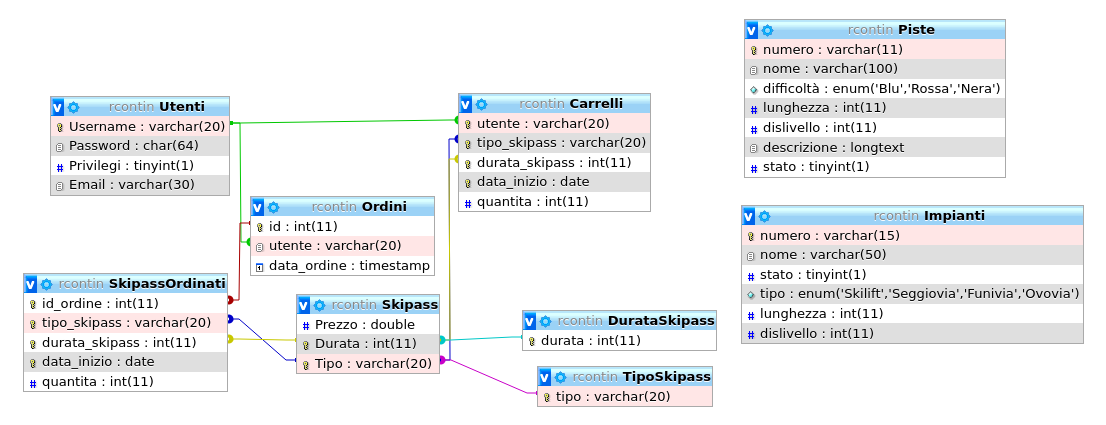
\includegraphics[width=\textwidth]{tabelle.png}



\subsection{Accessibilità}
Per avere un alto livello di accessibilità sono stati utilizzati i tag semantici dell'HTML5, dove necessario gli attributi WAI-ARIA e seguito lo standard WCAG 2.0.
\subsubsection{Separazione tra contenuto, presentazione e comportamento}
All'interno del sito sono state tenute divise:
\begin{itemize}
    \item 
        Il \textbf{contenuto} e la \textbf{struttura} sono stati codificati in HTML5 che a sua volta richiama i fogli di stile e gli script.;
    \item 
        La \textbf{presentazione} è definita in fogli di stile CSS3 multipli per adattarsi a qualsiasi tipo di dispositivo;
    \item 
        Il \textbf{comportamento} è sviluppato in JavaScript ed implementato in modo da rendere accessibili ed utilizzabili le pagine anche quando JavaScript disattivato.
\end{itemize}

\subsubsection{Navigazione}
La navigazione interna al sito è l'elemento la cui accessibilità è essenziale: se non fosse accessibile, tutto il resto perderebbe di importanza.
\paragraph{Link "Salta al contenuto"} Il link "Salta al contenuto" è un link che permette di spostare il focus dall'inizio della pagina direttamente al contenuto della stessa. Questo è uno strumento molto importante per chi fruisce del sito utilizzando solamente tastiera o dispositivi di input alternativi al mouse: la navigazione viene notevolmente velocizzata.

Il link è visibile solamente quando ha il focus, ed è contenuto all'interno di un tag \verb|<nav>| per denotarne la pertinenza. Inoltre l'utilizzo di \verb|aria-label| ne consente una esplicitazione della funzione parte di eventuali screen reader.

\paragraph{Menu principale}
Il Menu principale è una lista di links che portano ai contenuti del sito web. Anche in questo caso, è stato utilizzato il tag semantico \verb|<nav>| e l'attributo \verb|aria-label|.

È completamente navigabile senza l'ausilio del mouse, anche quando il menu risulta compresso, come nel caso del layout per schermi di medie dimensioni. Per assicurarsi che questo avvenga sono stati adottati i seguenti accorgimenti:
\begin{itemize}
    \item Uso di \verb|<button>|, che può prendere il focus da tastiera
    \item Utilizzo di \verb|aria-expanded| per segnalare o meno se il menu collegato è aperto
    \item \verb|aria-controls| per specificare che cosa si sta espandendo/comprimendo
    \item \verb|aria-label| per dare un \textit{feedforward} sull'azione che sta per avvenire.
\end{itemize}
\paragraph{Link "Scroll to top"}
Questo link ha funzione e realizzazione simili al link "Salta al contenuto". Permette di riportare il focus in cima alla pagina, è contenuto in un \verb|<nav>| e ha \verb|aria-label| per specificarne il comportamento.

\subsubsection{Form}
Al fine di mantenere accessibili tutti i form all'interno del sito, per ognuno di essi:
\begin{itemize}
    \item i valori immessi vengono controllati sia dal front-end utilizzando JavaScript che dal back-end con PHP con lo scopo di creare dei feedback di errore il più possibile utili all'utente ed in tempo reale;
    \item ogni campo di input è accompagnato da un tag <label> che lo descrive;
    \item in caso di successo dell'operazione a cui è collegato viene mostrato un feedback positivo.
\end{itemize}
